\chapter{관측, 암흑물질, 그리고 우주론적 적합}

\lectureoverview{관측은 우주론 모형과 연결될 때에만 의미를 얻는다. 프리드만 방정식과 세 가지 균질 공간 기하에서 출발해 현재 우주의 구성비를 복사, 물질, 진공 에너지, 곡률로 정리하고, 한때 열린 우주가 불가피해 보였던 이유를 재구성한다. 이어 은하 회전 곡선에서 중력을 일으키는 누락된 물질을 확인하고, 차갑고 약하게 상호작용하는 헤일로의 동역학을 살펴본다. 마지막으로 적색편이, 밝기, 천체 수를 통해 가정한 팽창 역사를 관측 가능한 곡선으로 바꾼다. 기존의 물질과 곡률만으로 된 모형은 관측과 맞지 않는다. 물질의 비율이 \(0.3\)에 가깝고, 진공의 비율이 \(0.7\)에 가까우며, 곡률이 매우 작은 모형이 이 강의에서 관측에 잘 맞는다.}

\section{관측을 다시 방정식에 대입하기}

천문학적 사실은 따로 떼어 놓고 해석할 수 없다. 어떤 관측량의 조합이 서로 다른 우주를 구별해 주는지 알려 주는 방정식이 먼저 필요하다. 균질하고 등방적인 우주에서는 프리드만 방정식이 출발점이다.
\begin{equation}
\left(\frac{\dot a}{a}\right)^2
=
\frac{8\pi G}{3}\rho-\frac{k}{a^2}.
\label{eq:c06-friedmann}
\end{equation}
양
\begin{equation}
H(t)=\frac{\dot a(t)}{a(t)}
\label{eq:c06-hubble}
\end{equation}은 허블 \emph{함수}이다. 현재 값 \(H_0\)은 관례상 허블 상수라고 부르지만, \(H(t)\)은 우주의 역사 내내 일정한 상수가 아니다. 천문학자들이 메가파섹당 초속 킬로미터 단위로 값을 제시할 때는 \(H_0\)을 제시하는 것이다.

정규화된 곡률 지표는 다음 세 값만 갖는다.
\begin{equation}
k\in\{+1,0,-1\},
\end{equation}
각 값은 차례로 구면, 평탄, 쌍곡 공간 기하에 해당한다. 흔히 쓰는 FRW 계량은 다음과 같이 쓸 수 있다.
\begin{equation}
ds^2=-dt^2+a(t)^2\left[dr^2+\xi(r)^2d\Omega_2^2\right],
\label{eq:c06-frw}
\end{equation}
여기서
\begin{equation}
\xi(r)=
\begin{cases}
\sin r, & k=+1,\\
r, & k=0,\\
\sinh r, & k=-1.
\end{cases}
\label{eq:c06-xi}
\end{equation}
이다. 이 표기법은 두 가지 역할을 한다. 세 가지 기하를 하나의 계량으로 나타내고, 뒤에서는 구의 면적을 주어 반지름 방향 껍질 안에 있는 천체의 수를 계산하게 해 준다. 따라서 \(k\)을 선택하고 \(a(t)\)에 대한 방정식을 정하는 것만으로도 관측 가능한 결과를 내는 모형이 된다.

\section{현재 우주의 구성비}

여기서 다루는 모형의 에너지 밀도에는 복사, 비상대론적 물질, 진공 에너지라는 세 가지 주요 성분이 있다. 곡률까지 같은 장부에 올리면 다음과 같다.
\begin{equation}
\frac{C_r}{a^4}
+\frac{C_m}{a^3}
+\Lambda
-\frac{k}{a^2}
=H^2.
\label{eq:c06-budget}
\end{equation}
여기서 \(\Lambda\)은 앞 강의의 정규화를 따른다. \(\Lambda=(8\pi G/3)\rho_{\rm vac}\) 복사는 \(a^{-4}\)에 따라, 물질은 \(a^{-3}\)에 따라 희석되고, 진공 에너지는 희석되지 않으며, 곡률 항은 \(a^{-2}\)에 따라 변한다. 곡률은 물질의 에너지 밀도가 아니지만, 다른 항들과 나란히 두면 현재의 제약 조건이 분명해진다. 네 기여분의 합은 \(H_0^2\)이어야 한다.

현재의 구성비를 다음과 같이 정의하자.
\begin{equation}
\begin{aligned}
\Omega_r&=\frac{C_r/a_0^4}{H_0^2},
&\qquad
\Omega_m&=\frac{C_m/a_0^3}{H_0^2},\\
\Omega_\Lambda&=\frac{\Lambda}{H_0^2},
&
\Omega_k&=\frac{-k/a_0^2}{H_0^2}.
\end{aligned}
\label{eq:c06-omegas}
\end{equation}
그러면
\begin{equation}
\boxed{\Omega_r+\Omega_m+\Omega_\Lambda+\Omega_k=1.}
\label{eq:c06-sum-rule}
\end{equation}
이다. \(\Omega\)들은 오늘 평가한 비율이지, 시간에 무관한 상수가 아니다. 부호 규약에도 유의하자. \(k=-1\)이면 \(\Omega_k\)은 양수다.

\subsection{처음 두 항은 어떻게 측정하는가}

허블은 후퇴 적색편이와 거리를 비교해 국소 팽창률을 구했다. 적색편이는 낮은 \(z\)에서 속도를 알려 주고, 보정된 밝기는 거리를 알려 준다. 그의 최초 수치는 크게 틀렸지만 방법은 옳았다. 은하들이 비교적 가까웠기 때문에 이 측정은 우주 역사의 큰 부분을 탐사하지 않았으며, \(H\)를 현재 값으로 취급할 수 있었다.

\begin{classroomqa}
\audiencequestion{천체의 고유 밝기를 이미 알고 있지 않다면 밝기로 어떻게 거리를 알아낼 수 있나요?}
\lecturerresponse{한 번에 알아낼 수는 없다. 우주 거리 사다리는 가까운 별의 연주시차에서 시작한다. 이처럼 보정된 영역에 있는 세페이드 변광성으로부터 주기와 광도의 관계를 알아내면, 더 먼 거리를 재는 표준촛불로 삼을 수 있다. 서로 겹치는 보정을 이어 사다리를 바깥으로 확장하고, 이후에 다룰 우주론적 적색편이 범위에서는 초신성이 가장 좋은 표준촛불이 된다. 따라서 거리는 모든 천체가 똑같이 빛난다는 자의적 가정이 아니라, 표준들을 잇는 단계적 과정을 통해 추론한다. \lecturetimestamp{00:10:00--00:11:32}}
\end{classroomqa}

\begin{classroomqa}
\audiencequestion{밀도가 변하는데도 \(C_r\)과 \(C_m\)은 상수인가요?}
\lecturerresponse{그렇다. 계수는 고정되어 있고, 시간에 따른 변화는 \(a^{-4}\)과 \(a^{-3}\)이 담당한다. 진공 에너지는 일정하고, 곡률 항은 \(a^{-2}\)에 따라 변한다. 이 서로 다른 거듭제곱 때문에 시대에 따라 각 성분의 비율이 달라진다. \lecturetimestamp{00:11:35--00:12:02}}
\end{classroomqa}

복사 항은 광자 배경을 국소적으로 측정해 구할 수 있다. 그 대부분은 우주 마이크로파 배경이며, 현재 에너지 밀도는 다른 주요 성분들에 비해 매우 작다. 충분히 큰 평균화 부피가 필요하지만, \(\Omega_r\)이 오늘날 무시할 수 있음을 확인하는 데 과거 광원뿔을 따라 멀리까지 나아갈 필요는 없다.

보이는 물질의 양은 은하, 항성 집단, 수소, 성간 가스를 바탕으로 추정한다. 방법은 기술적으로 까다롭지만 개념상 복잡하지는 않다. 별과 가스의 전형적인 양을 구하고, 은하 전체에 대해 합산한 다음, 큰 부피에 걸쳐 평균을 낸다. 이 강의에서는 대략적인 옛 기준으로 입방미터당 양성자 질량 하나를 든다. 복사 밀도보다 훨씬 크지만, 그래도 놀라울 만큼 희박하다.

\begin{classroomqa}
\audiencequestion{이 장부에서 암흑물질은 어떻게 다루나요?}
\lecturerresponse{곧 다루겠지만, 먼저 발광 물질만을 바탕으로 한 과거의 추론을 의도적으로 재구성한다. 역사적 순서가 중요한 까닭은 암흑물질이 어떤 겉보기 결론을 바로잡았고 어떤 간극은 메우지 못했는지 정확히 보여 주기 때문이다. \lecturetimestamp{00:15:08--00:15:40}}
\end{classroomqa}

\section{왜 한때 열린 우주가 불가피해 보였는가}

과거 모형에서는 복사가 무시할 만하다고 올바르게 판단했고, 진공 에너지는 0으로 두었으며, 물질은 전자기 복사를 통해 보이는 물질만을 뜻했다. 그러면 대략 다음과 같이 추정되었다.
\begin{equation}
\Omega_r\simeq0,
\qquad
\Omega_\Lambda=0,
\qquad
\Omega_m^{\rm luminous}\sim\frac{1}{20}\text{--}\frac{1}{30}.
\end{equation}
따라서 합 규칙은 다음을 강제하는 듯했다.
\begin{equation}
\Omega_k\simeq1.
\end{equation}
양의 곡률 기여분은 \(-k/a_0^2>0\)을 뜻하므로, 이는 \(k=-1\)을 함의했다. 즉 곡률이 음인 열린 우주다. 이 수치들은 과거의 논증을 재구성한 것이지, 현대적 모수 추정값은 아니다.

곡률의 규모를 해석하려면 물질이 지배하는 해로 돌아가자.
\begin{equation}
a(t)\propto t^{2/3}.
\end{equation}
이를 미분하고 \(a\)로 나누면
\begin{equation}
H(t)=\frac{\dot a}{a}=\frac{2}{3t}.
\label{eq:c06-matter-h}
\end{equation}
현재 나이 \(T\)에서는
\begin{equation}
H_0\simeq\frac{2}{3T}.
\end{equation}
이다. 따라서 허블 시간은 우주의 나이와 같은 차수다. 복사 지배 시대의 비교식
\begin{equation}
a(t)\propto t^{1/2},
\qquad
H(t)=\frac{1}{2t},
\end{equation}
을 보면 이 역수와 나이의 관계가 먼지에만 특유한 것은 아님을 알 수 있다.

\begin{figure}[htbp]
\centering
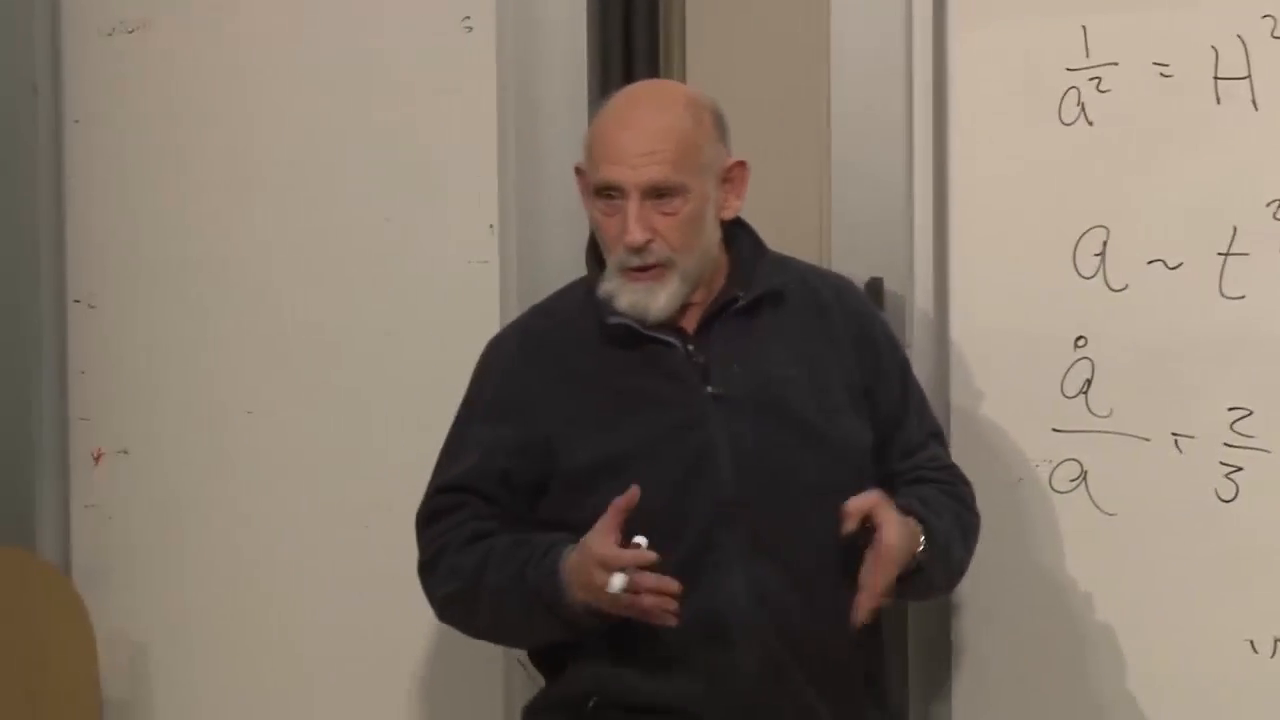
\includegraphics[width=0.72\textwidth]{lecture_06_figure_02.png}
\caption{물질 지배 시대를 판서로 복습하는 장면. 보이는 판서에는 \(a\sim t^{2/3}\)과 \(\dot a/a=2/(3t)\)이 있다. 강사가 나머지 판서 내용을 가리므로, 화면에서 확인할 수 없는 방정식을 이 장면의 내용으로 제시하지 않는다.}
\label{fig:c06-age-board}
\lectureframe{00:24:41.615}
\end{figure}

\begin{classroomqa}
\audiencequestion{허블 상수의 단위는 무엇이며, 빛의 속도는 어디에 들어가나요?}
\lecturerresponse{속도와 거리를 연결하는 \(H\)의 단위는 역시간이다. 초의 역수나 년의 역수로 표시할 수도 있고, 천문학자들이 쓰는 메가파섹당 초속 킬로미터 단위로 표시할 수도 있다. 관계식 \(H\sim1/T\)에는 별도의 \(c\)이 필요하지 않다. 시간 \(T\)을 \(cT\) 같은 길이로 환산할 때만 \(c\) 인자가 나타난다. \lecturetimestamp{00:22:50--00:24:25}}
\end{classroomqa}

허블이 최초로 구한 \(H_0\) 값은 실제보다 대략 한 자릿수 정도 컸고, 이에 해당하는 허블 나이는 강의에서 어림해 비교한 십억 년이 아니라 그보다 짧은 수십억 년 규모였다. 더 나은 보정으로 수치는 바로잡혔지만, \(H_0^{-1}\)이 우주적 시간 척도라는 논리는 바뀌지 않았다.

곡률에 관한 과거의 추론은 이제 다음과 같이 표현된다.
\begin{equation}
\frac{1}{a_0^2}\sim H_0^2\sim\frac{1}{T^2}.
\end{equation}
\(c=1\) 단위에서 곡률 반지름 \(a_0\)은 대략 우주의 나이 \(T\) 정도라고 여겨졌다. 보통 단위를 되살리면 대략 \(cT\) 정도다. 강의는 곧바로 이것이 실제 우주에 대한 진술은 아니라고 분명히 한다. 당시 무시할 만하다고 여긴 항들을 버리고 수십 년 전에 얻었던 결론을 말하는 것이다.

\begin{classroomqa}
\audiencequestion{오늘날 곡률이 지배적이어야 한다고 보면서 왜 물질 지배 법칙 \(a\propto t^{2/3}\)을 쓰나요?}
\lecturerresponse{물질 항은 \(a^{-3}\)에 따라 변하지만 곡률 항은 \(a^{-2}\)에 따라서만 변하기 때문이다. \(a\)가 작을수록 물질 항이 우세하다. 곡률은 우주 역사의 후기에야 중요해질 수 있으므로, 경과한 시간의 대부분은 여전히 물질 지배로 설명되며 \(H_0\)도 \(1/T\) 정도의 크기를 유지한다. 물질과 곡률을 함께 포함하는 완전한 해는 수치 계수를 보정하겠지만, 시간 척도에 관한 논증을 없애지는 않는다. \lecturetimestamp{00:49:20--00:50:17}}
\end{classroomqa}

\section{은하 동역학으로부터 암흑물질 추론하기}

물질의 양을 파악하는 데는 두 가지 방법이 있다. 하나는 빛을 방출하거나 흡수하는 물질을 세는 것이고, 다른 하나는 중력으로부터 질량을 추론하는 것이다. Oort는 1930년대 초에 은하의 비정상적인 동역학을 발견했고, Zwicky는 은하단에서 이에 상응하는 질량 불일치를 발견했다. 관측 증거는 중력에 기여하는 물질이 빛을 내는 물질보다 더 많다는 것을 보여 주었다. 보통의 전하를 띤 물질은 복사를 방출하고 충돌하지만, 누락된 성분은 처음에는 중력적 작용을 통해서만 알려졌다.

\begin{classroomqa}
\audiencequestion{발광 물질에 희박한 가스와 중심 블랙홀도 포함되나요?}
\lecturerresponse{희박한 가스는 전자기적 거동으로 양을 추론할 수 있는 만큼 포함된다. 중심의 초대질량 블랙홀도 알려진 질량 장부에 포함될 수 있지만, 은하 전체 질량에서 차지하는 비율은 작고 중심부에 집중되어 있다. 따라서 발광 중심부를 훨씬 벗어난 곳까지 이어지는 불일치를 설명할 수 없다. \lecturetimestamp{00:29:50--00:31:14}}
\end{classroomqa}

반지름 \(r\)인 원궤도를 거의 원형으로 도는 별을 생각해 보자. 질량 \(M\)의 거의 전부가 은하 중심 부근에 집중되어 있다면, 뉴턴 법칙에 따라
\begin{equation}
\frac{GM}{r^2}=\frac{v^2}{r},
\end{equation}
이므로
\begin{equation}
v^2=\frac{GM}{r},
\qquad
v(r)\propto r^{-1/2}.
\label{eq:c06-kepler}
\end{equation}
이 된다. 이는 중심 질량 분포 바깥에서 예상되는 케플러식 감소다.

\begin{figure}[htbp]
\centering
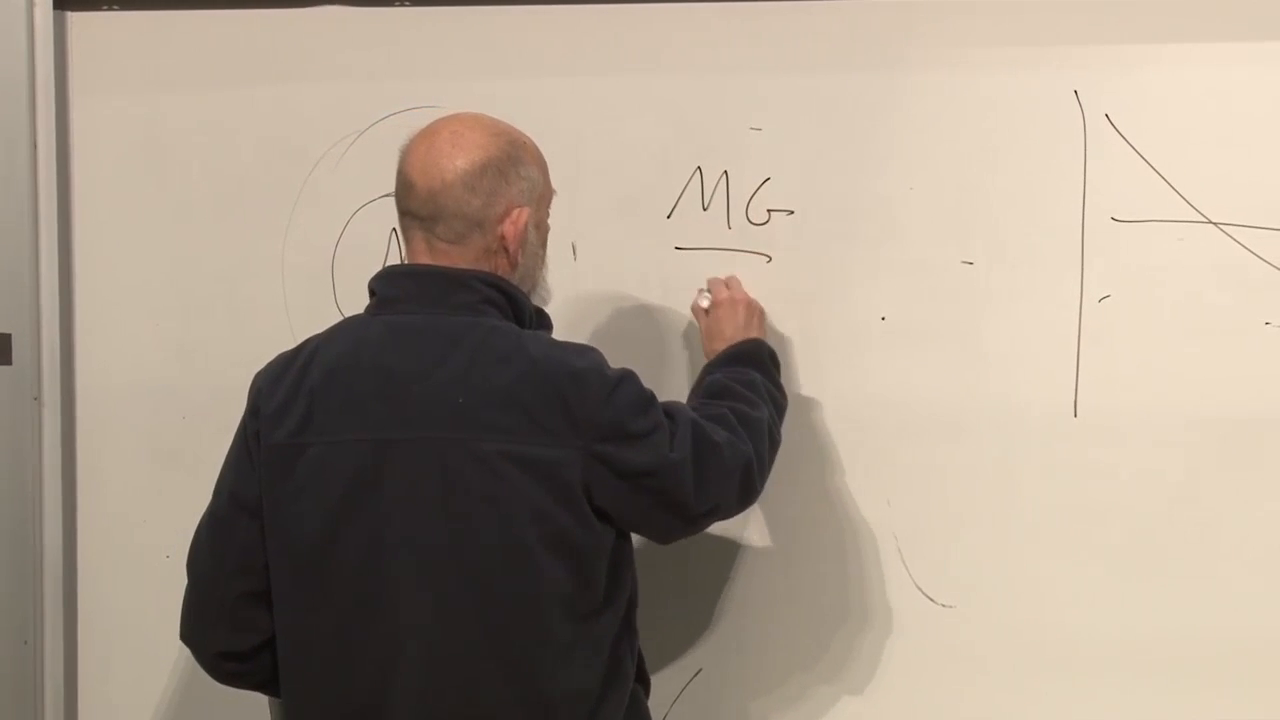
\includegraphics[width=0.78\textwidth]{lecture_06_figure_03.png}
\caption{중심 질량에서 내부 질량 \(M(r)\)으로 넘어가는 회전 곡선 판서. \(MG\), 분수선, 궤도 스케치, 곡선 스케치 일부만 보인다. 방정식~\eqref{eq:c06-kepler}은 강의 중 설명을 바탕으로 한 유도에서 나온다.}
\label{fig:c06-rotation-board}
\lectureframe{00:34:53.642}
\end{figure}

\begin{figure}[htbp]
\centering
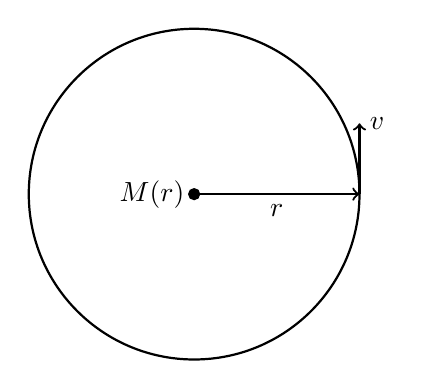
\begin{tikzpicture}[scale=1.0]
\filldraw (0,0) circle (2pt) node[left] {\(M(r)\)};
\draw[thick] (0,0) circle (2.1);
\draw[->,thick] (0,0)--(2.1,0) node[midway,below] {\(r\)};
\draw[->,thick] (2.1,0)--(2.1,0.9) node[right] {\(v\)};
\end{tikzpicture}
\caption{측정한 회전 속도에서 내부 질량을 추론하는 원궤도 구성.}
\label{fig:c06-orbit-redraw}
\end{figure}

관측된 은하 회전 곡선은 이런 식으로 감소하지 않는다. 상당한 반지름 범위에 걸쳐 거의 평탄하다. 고정된 중심 질량 대신 내부 질량 \(M(r)\)을 사용하면
\begin{equation}
\frac{G M(r)}{r^2}=\frac{v(r)^2}{r}.
\end{equation}
\(v(r)\)이 거의 일정할 때
\begin{equation}
\boxed{M(r)\propto r.}
\label{eq:c06-enclosed-mass}
\end{equation}
이 된다. 이는 국소 밀도가 아니라 반지름 \(r\) 안에 든 전체 질량을 뜻한다. 별빛 대부분이 집중된 영역을 훨씬 넘어 계속 중력 질량이 증가한다. 은하 원반에 수직인 운동도 대략 구형인 분포, 즉 얇은 원반이 하나 더 있는 것이 아니라 어두운 헤일로가 있다는 점을 뒷받침한다.

\begin{classroomqa}
\audiencequestion{회전 곡선이 왜 이렇게 평탄한지 설명하는 간단한 이론이 있나요?}
\lecturerresponse{이 논증에는 그런 설명이 없다. 은하 형성 시뮬레이션을 보면 이런 모양의 밀도 분포가 자연스럽게 나타날 수 있지만, 강의는 간단한 유도를 제시하지 않는다. 확실한 진술은 관측에 관한 것이다. \(v\)이 거의 일정하면 내부 질량은 대략 선형으로 증가한다. 이 관계가 깔끔하다는 사실을 은하 형성에 대한 초보적인 설명으로 오해해서는 안 된다. \lecturetimestamp{00:35:58--00:37:33}}
\end{classroomqa}

\begin{classroomqa}
\audiencequestion{나선팔은 각속도 \(v/r\)가 달라 생기는 물질의 바람개비 모양 구조인가요?}
\lecturerresponse{단순한 바람개비 모형으로는 설명할 수 없다. 눈에 보이는 패턴이 개별 별들과 함께 회전할 필요는 없다. 밀도파나 별 형성 파동으로 설명하는 것도 여러 가능성 가운데 하나다. 강의는 이 불확실성을 통해 신뢰할 만한 헤일로 추론과 더 복잡한 나선 구조 문제를 구분한다. \lecturetimestamp{00:37:35--00:38:34; 00:47:03--00:47:47}}
\end{classroomqa}

추론된 암흑 질량은 발광 질량의 몇 배이며, 이 강의에서는 대략 5배에서 10배 사이의 규모로만 제시한다. 헤일로는 눈에 보이는 은하보다 더 멀리까지 뻗어 있다. 이는 일부러 대략적으로 제시한 역사적 규모이지, 모든 계에 적용되는 정밀한 보편 비율은 아니다.

\section{암흑물질은 어떤 성질을 가져야 하는가}

보통 물질은 왜 밝고 조밀한 원반을 이루는 반면 암흑물질은 넓은 헤일로에 남아 있을까? 발광 물질은 전자기적 충돌과 복사를 통해 역학적 에너지를 잃을 수 있다. 에너지를 소산하고 나면 중력이 물질을 더 조밀한 구조로 끌어당길 수 있다. 암흑물질은 전기적으로 중성이며 상호작용이 훨씬 약한 것으로 보인다. 암흑물질 입자들은 충돌하거나 복사를 내는 일이 거의 없이 헤일로를 공전하므로, 수십억 년이 지나도 발광 원반에 가라앉을 만큼 충분한 에너지를 잃지 않는다. 은하 운동에서 나오는 중력 복사는 대안적 냉각 기작이 되기에는 너무 약하다.

\begin{classroomqa}
\audiencequestion{약하게 상호작용한다는 것은 암흑물질이 다른 중력 법칙을 따른다는 뜻인가요?}
\lecturerresponse{아니다. 암흑물질도 보통과 같은 방식으로 중력을 일으킨다고 가정한다. 여기서 약한 상호작용이란 중력이 아닌 충돌과 전자기 복사가 없거나 크게 억제되어 있음을 뜻한다. 암흑 입자 두 개도 서로 중력으로 끌어당긴다. 이 인력은 헤일로를 형성하지만 궤도 에너지를 효율적으로 소산시키지는 못한다. \lecturetimestamp{00:42:36--00:43:35}}
\end{classroomqa}

\begin{classroomqa}
\audiencequestion{이것이 특정 은하의 회전 곡선에서만 나타나는 특이 현상이 아님을 보여 주는 관측은 무엇인가요?}
\lecturerresponse{여러 규모에서 증거가 나타난다. 은하 안의 항성 운동, 은하 평면에 수직인 운동, 은하 간 상호작용, 은하단 전체의 동역학이 그 예다. 오르트와 츠비키의 사례는 같은 중력 질량 누락 문제가 서로 다르게 드러난 경우였다. \lecturetimestamp{00:42:00--00:42:36}}
\end{classroomqa}

\begin{classroomqa}
\audiencequestion{암흑물질은 블랙홀과 은하 중심에 모여야 하지 않나요?}
\lecturerresponse{중력 중심으로 갈수록 밀도는 높아지지만, 블랙홀이 먼저 존재하고 그 주변에 헤일로가 형성되었다기보다는 역사적 순서가 반대였을 가능성이 크다. 암흑 헤일로가 큰 중력 우물을 만들고, 그 뒤 중입자 물질이 그 안으로 떨어져 은하와 별, 중심 블랙홀을 형성했다. 블랙홀은 질량의 작은 부분을 차지한다. 그래도 암흑물질 소멸 생성물을 찾을 때는 은하 중심을 살펴보는데, 그곳의 암흑물질 밀도가 더 높으리라 예상하기 때문이다. \lecturetimestamp{00:43:36--00:45:43}}
\end{classroomqa}

\begin{classroomqa}
\audiencequestion{암흑물질은 기체, 먼지, 조밀한 덩어리, 아니면 고립된 입자인가요? 태양 근처에 일부가 붙잡혀 있을 수 있나요?}
\lecturerresponse{미시적 성질은 알려져 있지 않지만, 보통의 먼지는 전자기력에 묶여 있다. 이는 암흑물질에는 없는 듯한 바로 그런 상호작용이다. 따라서 기본 입자 모형에서는 개별 입자가 희박하게 분포한다고 본다. 일부는 태양 근처에 중력적으로 모여 있을 수 있지만, 밀도가 너무 낮아서 태양의 중력과 경쟁하거나 행성의 동역학을 교란할 수는 없다. \lecturetimestamp{00:45:43--00:47:02; 00:58:41--00:59:29}}
\end{classroomqa}

두 번째 핵심 조건은 암흑물질이 뭉칠 수 있어야 한다는 것이다. 상대론적 무작위 속도를 가진 뜨거운 입자 집단은 중력 응집에 저항하지만, 차가운 입자 집단은 퍼텐셜 우물로 떨어질 수 있다. 보통의 가벼운 중성미자는 뜨거운 암흑물질처럼 거동했을 것이므로, 필요한 주요 은하 성분이 될 수 없다. 여기서 \emph{차갑다}는 것은 우주론적 국소 기준계에서 비상대론적이라는 뜻이지, 실험실에서 문자 그대로 온도가 영이라는 뜻은 아니다.

\begin{classroomqa}
\audiencequestion{차가운 상태로 뭉쳐야 한다는 조건이 암흑물질의 질량 범위를 제한하나요?}
\lecturerresponse{양자 통계와 생성 이력에 따라 달라진다. 매우 가벼운 페르미온은 모두 느린 상태 하나를 차지할 수 없으므로 강한 제약을 받는다. 매우 가벼운 보손은 응집된 코히런트 보스 상태를 이룰 수 있으며, 강의에서는 액시온을 그 예로 든다. 또는 더 무거운 약상호작용 입자라면 응축하지 않아도 차가울 수 있다. 따라서 이 논증만으로는 모형에 무관한 단일 질량 한계를 제시할 수 없다. \lecturetimestamp{00:53:17--00:54:52; 00:56:42--00:58:05}}
\end{classroomqa}

\begin{classroomqa}
\audiencequestion{입자가속기에서 이미 그 입자들을 발견했어야 하지 않나요?}
\lecturerresponse{추가 가정을 해야만 그렇다. 입자의 약상호작용 단면적이 대략 예상되는 수준이고 질량이 가속기의 도달 범위 안에 있다면, 충돌기에서 생성될 가능성이 있다. 곧 정보를 얻을 수 있으리라는 강의의 기대는 명시적으로 추측이었고 당시 상황에 한정된 것이었다. 입자가 현재 실험으로는 다룰 수 없을 만큼 무겁거나 상호작용이 약할 수도 있다. \lecturetimestamp{00:54:52--00:55:54}}
\end{classroomqa}

\begin{classroomqa}
\audiencequestion{암흑물질은 단지 보이지 않는 여분의 차원에 있는 것일 수 있나요?}
\lecturerresponse{이 논의에는 그런 기작이 필요하지 않다. 암흑물질은 이미 중력 작용으로 관측되며, 보통 물질과 거의 상호작용하지 않는 특이한 입자일 수 있다. 상호작용이 약하다고 해서 입자들이 관측 가능한 시공간 바깥에 있다는 뜻은 아니다. \lecturetimestamp{00:55:54--00:56:41}}
\end{classroomqa}

보이지 않는 물질을 더하는 대신 중력을 수정하는 것은 논리적으로 가능한 대안이다. 강의에서는 당시 관련된 모든 규모의 증거를 설명하면서 태양계에서 검증된 법칙도 유지하는, 그만큼 간단한 수정 이론은 없다고 판단한다. 따라서 입자 해석을 더 선호하지만, 미시적 물리의 세부 사항은 여전히 알려져 있지 않다.

\section{암흑물질만으로는 과거의 우주 구성비 문제가 해결되지 않는다}

암흑물질을 포함하면 물질 기여분은 몇 배 커지지만, 발광 물질과 \(H_0^2\) 사이의 과거 불일치는 대략 25배 규모였다. 따라서 간극을 줄일 뿐 다음 식을 만족시키지는 못한다.
\begin{equation}
\frac{C_m}{a_0^3}=H_0^2.
\end{equation}
과거의 진공 에너지 없는 \(\Lambda\) 모형에서는 곡률 예산 항이 양수여야 했고, 따라서 \(k<0\)이어야 했다. 그런 열린 모형에 논리적 모순이 있었던 것은 아니다. 핵심은 암흑물질만으로 현대의 답을 선택할 수 없었다는 점이다.

\begin{classroomqa}
\audiencequestion{현대적 적합이 나오기 전 우주론자들은 곡률을 어떻게 생각했나요?}
\lecturerresponse{증거는 혼란스러웠고, 닫히고 유한한 우주를 선호하는 기존 관점이 물질 구성비와 충돌하기도 했다. 과거의 가정들을 일관되게 결합하면 음의 곡률이 자연스러운 추론이었다. 다만 암흑물질과 진공 에너지를 오늘날처럼 확실히 포함한 것이 아니었으므로, 당시의 역사적 합의는 잠정적이었다. \lecturetimestamp{00:50:17--00:51:50}}
\end{classroomqa}

따라서 후보 모형의 진실성을 우주 구성비에 관한 한 줄의 식만으로 추론할 것이 아니라 검증해야 한다. 모형은 곡률의 선택 \(k\)과 팽창 역사 \(a(t)\)로 이루어진다. 이는 물질의 상태 방정식과 현재 모수의 집합으로 나타낼 수도 있으며, 이로부터 \(a(t)\)를 계산한다. 과거의 후보 모형은 복사가 무시할 만큼 작고 우주 상수가 없는, 물질과 음의 곡률만으로 이루어진 모형이다.

\section{기하를 관측량으로 바꾸기}

\subsection{고정된 기하에서 천체 수와 밝기}

우주 진화를 잠시 무시하자. 균질한 우주에서 공변 껍질 안의 천체 수는 그 면적에 비례한다.
\begin{equation}
dN\propto \xi(r)^2\,dr.
\label{eq:c06-shell-count}
\end{equation}
따라서
\begin{equation}
dN\propto
\begin{cases}
\sin^2r\,dr, & k=+1,\\
r^2\,dr, & k=0,\\
\sinh^2r\,dr, & k=-1.
\end{cases}
\end{equation}
큰 \(r\)에서 음의 곡률인 경우는 \(\sinh^2r\sim e^{2r}\)처럼 증가하여 평탄한 경우의 법칙 \(r^2\)보다 훨씬 빠르다. 그러므로 음의 곡률은 거리가 커질수록 천체 수가 이례적으로 빠르게 증가한다고 예측한다.

같은 면적은 관측되는 플럭스에도 영향을 준다. 평탄한 정적 공간에서 표준 광원이 주는 플럭스는
\begin{equation}
F\propto\frac{1}{r^2}.
\end{equation}
이다. 쌍곡 공간에서는 복사가 퍼지는 구의 면적이 더 빠르게 증가하므로 플럭스는 더 빠르게 감소한다. 이 강의에서는 때때로 이 관측량을 광도라고 부르지만, 여기서 \(F\)은 겉보기 밝기 또는 플럭스를 뜻하고 고유 광도는 광원 자체의 값이다. 따라서 천체 수와 밝기를 함께 보면 공간 기하를 구별할 수 있다.

\subsection{적색편이와 과거 광원뿔}

실제 우주는 진화하며, 더 멀리 본다는 것은 더 과거를 본다는 뜻이다. \(t_{\rm em}\)에 방출된 빛은 스케일 인자가 \(a(t_{\rm em})\)에서 \(a_0\)까지 커지는 동안 늘어난다.
\begin{equation}
1+z
=\frac{\lambda_{\rm obs}}{\lambda_{\rm em}}
=\frac{a_0}{a(t_{\rm em})}.
\label{eq:c06-redshift}
\end{equation}
이를 다음과 같이 쓸 수도 있다.
\begin{equation}
z=\frac{\lambda_{\rm obs}}{\lambda_{\rm em}}-1.
\end{equation}
우리의 과거 광원뿔 위에 있는 서로 다른 점들은 서로 다른 공변 반지름과 방출 시각에 동시에 대응한다. 팽창은 파장을 변화시킨다. 도플러 편이와 중력 편이도 다른 물리적 기작이지만, 여기서 다루는 효과는 우주 팽창이다.

\begin{classroomqa}
\audiencequestion{적색편이 \(z\)의 정의에 왜 1을 빼나요?}
\lecturerresponse{편이가 없는 광원이 \(z=0\)을 갖도록 정한 역사적 관례다. 물리적으로 직접적인 늘어남의 비율은 \(1+z=\lambda_{\rm obs}/\lambda_{\rm em}\)이다. \lecturetimestamp{01:10:11--01:10:45}}
\end{classroomqa}

방사 방향 빛에서는 \(d\Omega_2=0\)이고 \(ds^2=0\)을 따른다. 따라서 방정식~\eqref{eq:c06-frw}은 다음을 준다.
\begin{equation}
dt^2=a(t)^2dr^2.
\end{equation}
우리에게 들어오는 광선을 따라 현재부터 과거 방향으로 거슬러 올라가면
\begin{equation}
dt=-a(t)\,dr,
\qquad
\frac{dr}{dt}=-\frac{1}{a(t)}.
\label{eq:c06-null-ray}
\end{equation}
이다. 마이너스 부호는 광선을 따라 더 큰 공변 반지름이 더 이른 시각에 놓인다는 뜻이다. \(a(t)\)를 알면 이 방정식으로 \(r(t)\)를 구할 수 있다.

\subsection{적색편이 단위당 천체 수}

관측자는 적색편이 구간 \(z\)부터 \(z+dz\)까지에 속하는 표준 광원들을 셀 수 있다. 먼저 방정식~\eqref{eq:c06-shell-count}에서 출발해 과거 광선을 따라 방정식~\eqref{eq:c06-redshift}을 미분하자.
\begin{equation}
dz=-\frac{a_0}{a^2}\,da
=-\frac{a_0}{a^2}\dot a\,dt.
\end{equation}
\(dt=-a\,dr\)를 사용하면
\begin{equation}
dz=\frac{a_0}{a}\dot a\,dr
=(1+z)\dot a\,dr.
\end{equation}
이다. 따라서
\begin{equation}
dr=\frac{dz}{(1+z)\dot a},
\end{equation}
이며, 공변 천체 밀도가 일정하다면
\begin{equation}
\boxed{
\frac{dN}{dz}
\propto
\frac{\xi(r)^2}{(1+z)\dot a}
}.
\label{eq:c06-dndz}
\end{equation}
이 된다. 강의 중 유도에서는 부호와 인자를 여러 차례 확인한다. 방정식~\eqref{eq:c06-null-ray}과 \eqref{eq:c06-redshift}을 보면 결과가 명확히 정해진다.

\begin{figure}[htbp]
\centering
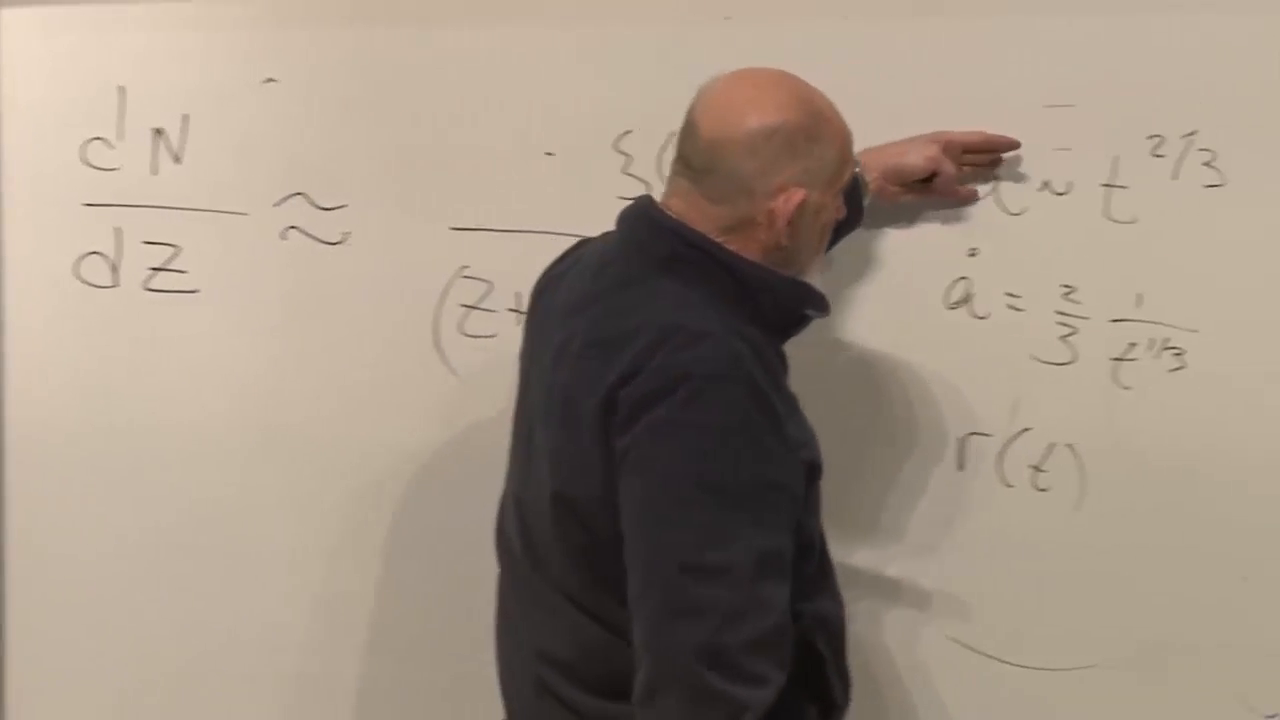
\includegraphics[width=0.84\textwidth]{lecture_06_figure_05.png}
\caption{모형 함수들과 \(dN/dz\)의 관계를 나타낸 판서. 왼쪽 항과 오른쪽의 \(a\sim t^{2/3}\), \(\dot a\), \(r(t)\)은 보이지만, 강사가 분모 일부를 가린다. 방정식~\eqref{eq:c06-dndz}은 앞서 독립적으로 유도했다.}
\label{fig:c06-dndz-board}
\lectureframe{01:22:24.114}
\end{figure}

모형을 선택하기 전에는 더 계산할 것이 없다. \(a(t)\)를 지정하면 \(\dot a(t)\)가 정해지고, 방정식~\eqref{eq:c06-null-ray}으로 \(r(t)\)를 구하며, 방정식~\eqref{eq:c06-redshift}을 사용하면 모든 양을 \(z\)의 함수로 나타낼 수 있다. 서로 다른 상태 방정식은 서로 다른 함수 \(dN/dz\)와 \(F(z)\)를 만든다. 바로 이 점 때문에 관측량으로 모형들을 판별할 수 있다.

\section{가정한 모수에서 최적 적합까지}

절차는 간단하다.
\begin{equation}
(\Omega_r,\Omega_m,\Omega_\Lambda,\Omega_k)
\longrightarrow
a(t)
\longrightarrow
\left\{F(z),\frac{dN}{dz}\right\}.
\label{eq:c06-fit-pipeline}
\end{equation}
현재 모수를 정하고, 프리드만 방정식을 풀고, 방사 방향 빛의 진행을 계산한 다음, 적색편이에 따른 밝기와 천체 수를 구해 관측 자료와 비교한다. 비교에 실패하면 그 모수 집합을 기각한다. 두 관측량을 함께 사용하면 팽창 역사와 공간 기하를 모두 제약할 수 있다.

\begin{figure}[htbp]
\centering
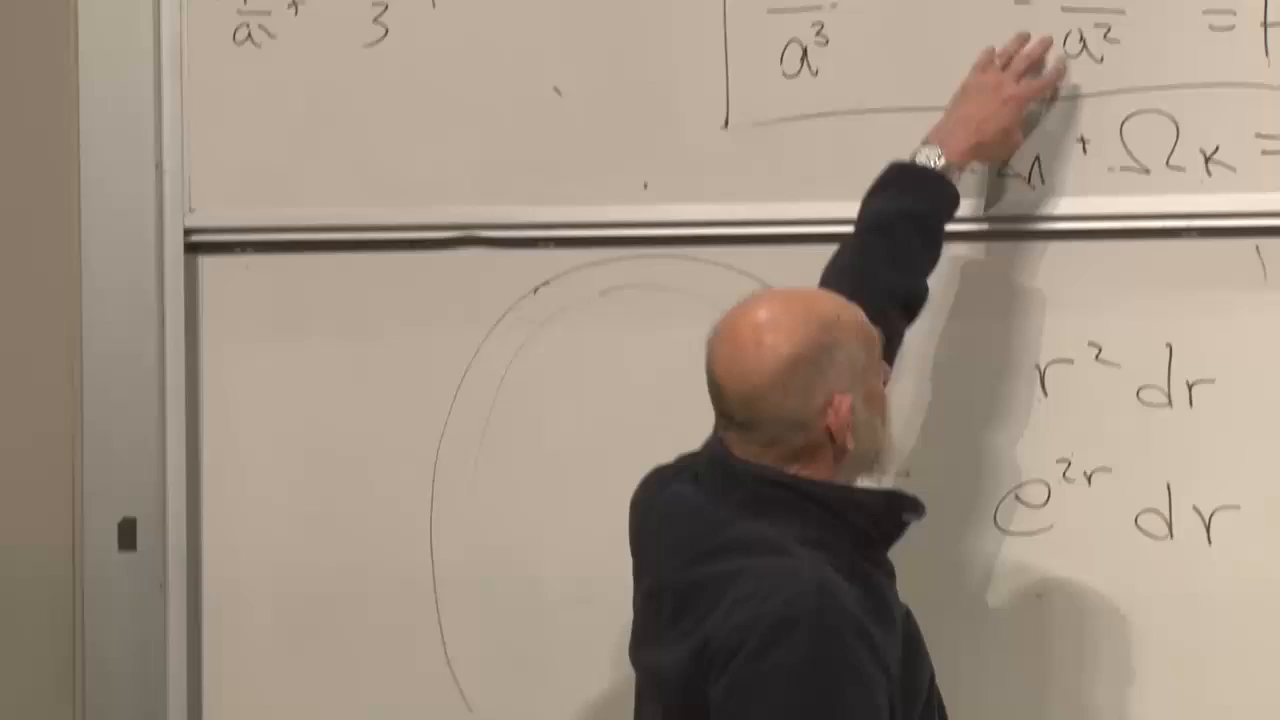
\includegraphics[width=0.84\textwidth]{lecture_06_figure_06.png}
\caption{위쪽 판서에는 과거의 물질과 곡률 모형이, 아래쪽 판서에는 평탄 및 쌍곡 껍질 인자 \(r^2dr\)과 \(e^{2r}dr\)이 있다. 프리드만 방정식 일부가 가려져 있으므로, 이 장면은 방정식의 근거라기보다 보조 자료다.}
\label{fig:c06-old-model-board}
\lectureframe{01:24:27.863}
\end{figure}

과거 모형
\begin{equation}
H^2=\frac{C_m}{a^3}-\frac{k}{a^2},
\qquad k=-1,
\end{equation}
은 밝기와 적색편이의 관계 및 천체 수 검증 모두에 맞지 않는다. 관련 적색편이 범위에서는 초신성이 가장 유용한 표준촛불이다. 이 강의에서 관측에 가장 잘 맞는 모수 집합은 다음과 같다.
\begin{equation}
\boxed{
\Omega_r\simeq0,\qquad
\Omega_m\simeq0.3,\qquad
\Omega_\Lambda\simeq0.7,\qquad
\Omega_k\simeq0
}.
\label{eq:c06-best-fit}
\end{equation}
여기서 물질에는 발광 물질과 암흑물질이 모두 포함된다. 이 값은 강의 당시의 적합 결과를 나타낸다. 오래 유지될 교훈은 적합 방법과 희석되지 않는 성분이 지배적이어야 한다는 점이지, 마지막으로 인쇄된 소수점 자릿수가 아니다.

\subsection{측정량과 적합량에 관한 질문}

\begin{classroomqa}
\audiencequestion{과거의 열린 우주 모형을 논의할 때 이미 \(\Lambda\)을 가정했나요?}
\lecturerresponse{아니다. 앞부분에서는 의도적으로 \(\Lambda=0\)인 과거 모형을 재구성했다. 방정식~\eqref{eq:c06-best-fit}의 값은 이후의 현대적 적합 결과를 나타낸다. 과거의 후보 모형을 아무 설명 없이 수정한 것이 아니라, \(F(z)\)와 \(dN/dz\)에 대조해 검증했고, 그 결과 맞지 않았다. \lecturetimestamp{01:26:45--01:27:07}}
\end{classroomqa}

\begin{classroomqa}
\audiencequestion{진공 에너지를 국소 물질처럼 직접 측정할 수 없다면 \(\Omega_\Lambda\)은 어떻게 구하나요?}
\lecturerresponse{먼저 시험할 모수 집합들을 정한다. 각각은 프리드만 해를 규정하고, 그에 따라 예측 함수 \(F(z)\)와 \(dN/dz\)를 정한다. 그 예측을 관측과 비교해 적합도가 낮은 집합을 버리고 모수 공간에서 가장 잘 맞는 영역을 남긴다. \(0.7\)은 진공 에너지 측정기로 직접 읽은 값이 아니라 적합에서 추론한 값이다. \lecturetimestamp{01:27:08--01:29:59; 01:31:57--01:33:40}}
\end{classroomqa}

\begin{classroomqa}
\audiencequestion{현재 스케일 \(a_0\)은 어디서 비롯되는가?}
\lecturerresponse{\(a\)의 정규화에는 관례에 따른 부분이 있지만, \(H_0\)에 연결된 완성된 모형은 \(k\ne0\)일 때 현재의 물리적 곡률 스케일을 제공한다. 모형이 적색편이 관측량에 들어맞으면, 그 함수 \(a(t)\)가 현재 시점과 이에 대응하는 스케일을 정해 준다. \lecturetimestamp{01:29:59--01:30:42}}
\end{classroomqa}

\begin{classroomqa}
\audiencequestion{수십억 년 전을 내다보면 오늘날의 매개변수에 기반한 적합이 왜곡되는가?}
\lecturerresponse{과거를 들여다보는 것은 왜곡이 아니라 신호다. 오늘날의 매개변수를 프리드만 방정식에 대입하면, 방정식은 이를 시간에 따라 진화시켜 완전한 \(a(t)\)을 산출한다. 예측된 광원뿔에는 작은 \(a\)에서 물질의 영향이 더 컸다는 사실이 이미 반영되어 있으며, 충분히 과거로 거슬러 올라가면 복사가 지배한다. 이러한 진화를 무시한 모형은 관측 자료와 맞지 않을 것이다. \lecturetimestamp{01:30:43--01:31:55}}
\end{classroomqa}

\begin{classroomqa}
\audiencequestion{현재의 어떤 물리량을 비교적 직접 측정하는가?}
\lecturerresponse{복사 밀도는 측정되며, 오늘날에는 무시할 만큼 작다. 허블 팽창률은 거리-적색편이 관계로부터 측정한다. 총 물질 밀도는 발광 물질과 암흑 물질을 모두 포함해 중력 효과로 추론한 뒤, 임계 스케일 \(3H_0^2/(8\pi G)\)로 나누어 \(\Omega_m\)을 얻는다. 후기 우주에서 남는 자유도는 주로 진공 에너지와 곡률에 있다. \lecturetimestamp{01:33:40--01:35:32}}
\end{classroomqa}

\begin{classroomqa}
\audiencequestion{\(\Omega_\Lambda\)와 \(\Omega_k\)를 모두 모르는 경우, \(\Omega_m\)를 고정하면 왜 후기 우주의 독립적인 시험 매개변수는 하나뿐인가?}
\lecturerresponse{방정식~\eqref{eq:c06-sum-rule}이 하나의 제약 조건을 부과하기 때문이다. \(\Omega_r\)가 무시할 만큼 작고 \(\Omega_m\)가 측정된 상태에서, 시험값 \(\Omega_\Lambda\)를 택하면 남은 \(\Omega_k=1-\Omega_m-\Omega_\Lambda\)가 정해진다. 곡률을 매개변수로 삼아 같은 1차원 모형군을 나타내도 된다. 예를 들어, \(\Omega_m=0.3\)일 때 \(\Omega_\Lambda=0.4\)와 \(\Omega_k=0.3\)는 유효한 시험값이다. 이 값이 기각되는 이유는 예측 곡선이 관측에 잘 들어맞지 않기 때문이지, 합 규칙이 이를 금지하기 때문이 아니다. \lecturetimestamp{01:35:33--01:39:09}}
\end{classroomqa}

\begin{classroomqa}
\audiencequestion{\(k\)는 이산적인 \(+1,0,-1\) 값만 취하는데 \(\Omega_k\)는 어떻게 연속적으로 변할 수 있는가? 차원은 올바른가?}
\lecturerresponse{이산적인 \(k\)는 부호와 정규화된 기하만 나타낸다. 연속적으로 변하는 곡률 반경은 \(a_0\)가 담고 있으므로 \(-k/(a_0^2H_0^2)\)는 연속적인 값들을 취할 수 있다. 단위계 \(c=1\)에서는 역길이와 역시간의 차원이 같다. 관례적인 단위를 복원하면 필요한 \(c\)의 거듭제곱이 붙는다. \lecturetimestamp{01:39:10--01:40:07}}
\end{classroomqa}

\begin{classroomqa}
\audiencequestion{은하 집단은 진화하는데도 개수 세기 방법은 균질성과 등방성을 가정하는가?}
\lecturerresponse{이 방법은 충분히 큰 공간 단면에서 균질성과 등방성을 가정하며, 같은 적색편이에서 서로 다른 방향을 비교해 이러한 대칭성을 검증할 수 있다. 광원 집단의 진화는 별개의 문제다. 서로 다른 시대의 집단이 같을 필요는 없으므로, 실제 분석에서는 수밀도가 영원히 일정한 것처럼 가정하지 않고 선택 효과와 진화를 모형화한다. 간단한 유도에서는 이러한 보정을 더하기에 앞서 기하학적 인자를 따로 살펴본다. \lecturetimestamp{01:40:08--01:41:08}}
\end{classroomqa}

\section{밀도 매개변수의 시간 변화}

방정식~\eqref{eq:c06-budget}은 모든 시간에 성립하지만, 방정식~\eqref{eq:c06-omegas}의 \(\Omega\)들은 현재 시각을 기준으로 정의되었다. 이에 대응하는 시간 의존량은 네 항이 \(a\)의 서로 다른 거듭제곱에 비례하므로 변한다. 아주 먼 과거에는,
\begin{equation}
\Omega_r(t)\longrightarrow1.
\end{equation}
복사는 더 빠르게 희석되므로 물질의 비중은 점차 커져 지배적인 성분에 가까워진다. 이후 \(\Lambda\)가 일정하게 유지되는 동안 물질 자체도 희석되므로, 아주 먼 미래에는,
\begin{equation}
\Omega_\Lambda(t)\longrightarrow1.
\end{equation}
따라서 물질 분율은 처음에는 작고 물질 시대에는 단위값에 가까워졌다가, 진공 에너지가 우세해진 뒤 다시 감소한다. 곡률이 0이 아니라면 곡률의 영향도 결국 양의 상수 \(\Lambda\)에 비해 작아진다.

\begin{classroomqa}
\audiencequestion{현재 곡률 분율이 작다는 것은 우주가 팽창하면서 더 평탄해진다는 뜻인가?}
\lecturerresponse{물리적 곡률 스케일은 \(a\)에 따라 커지고, 양의 우주 상수에 견주면 곡률 기여분 \(a^{-2}\)은 점점 덜 중요해진다. 이것이 \emph{큰 규모에서는 평탄하다}라는 표현의 의미다. 이 현상은 이산적인 위상 표지 \(k\)를 바꾸지 않는다. 국소 곡률과 동역학에서 곡률이 차지하는 분율이 감소한다는 뜻이다. \lecturetimestamp{01:47:13--01:47:42}}
\end{classroomqa}

\begin{classroomqa}
\audiencequestion{적합된 모형에서 설명되지 않는 체계적인 잔차가 나타났나요? 그 주장의 정밀도는 어느 정도였나요?}
\lecturerresponse{강의에서는 그 수준에서 이 체계에 알려진 체계적 실패가 없다고 보고하며, 이를 퍼센트 수준의 정밀 우주론이라고 설명한다. 퍼센트의 십분의 일이나 백분의 일 수준의 정밀도라는 뜻은 아니다. 이 진술은 당시의 상황에 관한 것이므로, 변하지 않는 현재의 오차 범위로 해석해서는 안 된다. \lecturetimestamp{01:45:40--01:46:19}}\end{classroomqa}

\begin{classroomqa}
\audiencequestion{초신성의 밝기와 개수를 이용하는 방법뿐 아니라 직접 삼각측량으로도 공간 곡률을 검증할 수 있는가?}
\lecturerresponse{그렇다. 우주 마이크로파 배경의 각도 분포는 표준 물리적 스케일을 제공하므로, 이를 이용해 거대한 우주 삼각형을 구성할 수 있다. 초신성 자료만으로는 강의에서 말한 퍼센트 수준의 곡률 정밀도를 얻지 못했다. 초신성 자료를 마이크로파 배경의 기하 정보와 결합하면 검증이 더 정밀해진다. 이것이 다음 강의의 주제다. \lecturetimestamp{01:46:19--01:47:12}}
\end{classroomqa}

\section{기억해 둘 핵심}

핵심 교훈은 네 가지 숫자의 목록이 아니라 하나의 방법이다. 우주론적 매개변수 집합은 \(a(t)\)를 정하고, 계량은 빛의 전파, 광원의 밝기, 광원 수를 예측한다. 관측과의 일치는 선택한 매개변수와 이를 연결하는 프리드만 이론 틀을 모두 검증한다. 임의로 고른 매개변수 집합이 관측에 들어맞으리라는 보장은 없다.

기존의 발광 물질과 음의 곡률을 가정한 모형은 관측과 맞지 않았다. 암흑 물질을 도입하면 중력을 일으키는 물질의 목록은 보완되지만, 그것만으로는 기존 프리드만 예산의 부족분이 해소되지 않았다. 강의 당시 관측에 성공적으로 들어맞은 모형에는 대략 다음 값이 필요했다.
\begin{equation}
\Omega_m\simeq0.3,
\qquad
\Omega_\Lambda\simeq0.7,
\qquad
\Omega_k\simeq0,
\end{equation}
곡률을 정밀하게 측정하는 데는 마이크로파 배경이 중요한 역할을 했다. 여러 독립적인 관측 결과를 하나의 동역학 이론에 적용했을 때, 매개변수 공간의 같은 영역에서 서로 부합한다는 점이 이 모형에 신뢰성을 부여한다.
